\documentclass[a4paper,10pt]{article}
%\usepackage[english]{babel}   % se si scrive in inglese
\usepackage[italian]{babel}       % se si scrive in italiano
\usepackage[T1]{fontenc}       % serve per la codifica delle lettere accentate (per evitare di scrivere \`e) 
\usepackage[utf8]{inputenc}   % serve per la codifica delle lettere accentate (per evitare di scrivere \`e)

\usepackage{graphicx}  % per includere le figure
\usepackage{rotating}   
\usepackage{lscape}
\usepackage{amsmath}
\usepackage{mathrsfs}
\usepackage[abs]{overpic}
\usepackage{color}
\usepackage{layout}
\usepackage[textwidth=16cm,textheight=24cm]{geometry} 

\usepackage{hyperref}

%% Definizione di nuovi commandi %%%
\newcommand{\latex}{\LaTeX}
\newcommand{\CP}{{\rm CP}}
\newcommand{\proton}{\ensuremath{p}}
\newcommand{\antiproton}{\ensuremath{\bar{p}}}
\newcommand{\acp}{\ensuremath{{\cal A}_{\CP}}}
\newcommand{\Lbppi}{\ensuremath{\Lambda_{b}^{0} \rightarrow p\pi^{-}}}
\newcommand{\aLbppi}{\ensuremath{\bar{\Lambda}_{b}^{0} \rightarrow \bar{p}\pi^{+}}}
\newcommand{\acplbppi}{\ensuremath{\acp(\Lbppi)}}
\newcommand{\lambdazero}{\ensuremath{\Lambda}}
\newcommand{\alambdazero}{\ensuremath{\bar{\Lambda}}}
\newcommand{\lambdazeroppi}{\ensuremath{\lambdazero \to \proton\pi^-}}
\newcommand{\alambdazeroppi}{\ensuremath{\bar{\lambdazero} \to \antiproton \pi^+}}

\newcommand{\pt}{\ensuremath{p_{\rm{T}}}}
\newcommand{\lxy}{\ensuremath{L_{\rm{T}}}}
\newcommand{\pdf}{\ensuremath{\wp}}

\newcommand{\mum}{\mbox{$\mu$m}}				%	um
\newcommand{\mus}{\mbox{$\mu$s}}
\newcommand{\tev}{\ensuremath{\mathrm{Te\kern -0.1em V}}}
\newcommand{\gev}{\ensuremath{\mathrm{Ge\kern -0.1em V}}}	%	GeV
\newcommand{\mev}{\ensuremath{\mathrm{Me\kern -0.1em V}}}	%	MeV
\newcommand{\kev}{\ensuremath{\mathrm{ke\kern -0.1em V}}}	%	keV
\newcommand{\massgev}{\mbox{\gev/$c^2$}}			%	GeV/c^2
\newcommand{\massmev}{\mbox{\mev/$c^2$}}			%	MeV/c^2
\newcommand{\pgev}{\mbox{\gev/$c$}}				%	GeV/c
\newcommand{\pmev}{\mbox{\mev/$c$}}				%	MeV/c

\newcommand{\note}[1]{\textcolor{red}{#1}}

%%%%%%%%%%%%%%%%%%%%%%%%%%
%%%%%% BEGIN DOCUMENT %%%%
%%%%%%%%%%%%%%%%%%%%%%%%%%
\begin{document}
\begin{flushright}             
\today
\end{flushright} 

\begin{center}
\Large{\bf Condizioni di lavoro di un contatore a scintillazione. }

\vspace*{1cm}                                 
\large{Michael Denuccio, Fabio Spagliardi, Giacomi Vitali, Salvatore Zaza }\\ 
\vspace*{0.5cm}       
\vspace*{1.cm}
\end{center}

%{ \abstract  
%}


\section{Introduzione}
\label{sec:intro} 
Lo scopo dell'esperienza è quello di acquisire pratica e mettere a punto un sistema di tre rilevatori a scintillatore plastico. Infine valutare un opportuno punto di lavoro per poi misurare l'efficienza di uno dei tre.

%%%%%%%%%%%%%%%%%%%%%%%%%%%%%%%%%%%%%%%%%%%%%%%%%%%%%%%%%%%%%%%%%%%%%%%%%%%%%%%%
%%%%%%%%%%%%%%%%%%%%%%%%%%%%%%%%%%%%%%%%%%%%%%%%%%%%%%%%%%%%%%%%%%%%%%%%%%%%%%%%
%%%%%%%%%%%%%%%%%%%%%%%%%%%%%%%%%%%%%%%%%%%%%%%%%%%%%%%%%%%%%%%%%%%%%%%%%%%%%%%%
\section{Raggi cosmici}
\note{Un po' di teoria sui raggi cosmici e una giustificazione sul numero di muoni attesi}

\section{Apparato Sperimentale}
In figura \ref{fig:none} è schematizzano l'apparato sperimentale. \`E composto da tre scintillatori collegati tramite una guida d'onda ad un fotomoltiplicatore (PMT). Faremo riferimento ai 3 tramite il numero associato al loro PMT (come in figura).
\\I PMT sono alimentati tramite un modulo dell'alta tensione (HV). 
\\Per l'osservazione e l'acquisizione dei segnali dai PMT abbiamo utilizzato i seguenti strumenti elettronici:
\begin{itemize}
\item Multimetro digitale;
\item Oscilloscopio a 2 canali;
\item Modulo FAN-IN FAN-OUT per lo smistamento dei segnali;
\item Discriminatore NIM a 8 canali;
\item Diversi moduli per il delay dei segnali;
\item Un modulo NIM per le coincidenze;
\item Un contatore digitale NIM con timer;
\end{itemize}


\label{sec:apparato} 
\subsection{Scintillatore Plastico}
Uno scintillatore plastico è composto da una lastra di materiale organico capace di emettere fotoni quando viene attraversato da una particella ionizzante. 

\subsection{PhotoMultiplier Tube (PMT)}

\subsection{Elettronica di Front-End}


%%%%%%%%%%%%%%%%%%%%%%%%%%%%%%%%%%%%%%%%%%%%%%%%%%%%%%%%%%%%%%%%%%%%%%%%%%%%%%%%
%%%%%%%%%%%%%%%%%%%%%%%%%%%%%%%%%%%%%%%%%%%%%%%%%%%%%%%%%%%%%%%%%%%%%%%%%%%%%%%%
%%%%%%%%%%%%%%%%%%%%%%%%%%%%%%%%%%%%%%%%%%%%%%%%%%%%%%%%%%%%%%%%%%%%%%%%%%%%%%%%


\section{Ricerca del punto di lavoro}
\label{sec:puntodilavoro} 
\subsection{Calibrazione del discriminatore e del contatore}
\note{descrivere la misura effettuata sul trigger del discriminatore e il controllo del timer del contatore}

\subsection{Osservazioni preliminari}
Inizialmente abbiamo alimentate il PMT4 con una tensione di 1.700 V, osservando un assorbimento in corrente di 0,693 mA. Collegando il segnale all'oscilloscopio ed impostando una soglia di trigger di 30 mV abbiamo visualizzato impulsi della durata dai 25 ai 31 ns, di ampiezza molto variabile dai 30 ai 750 mV, ad una frequenza dell'ordine dei kHz.
\\
Quindi abbiamo collegato il PMT ad un contatore tramite un discriminatore, impostato con una soglia a 50mV e una larghezza del segnale di uscita di 40ns. In questo modo abbiamo preso le misure mostrate nel grafico \ref{fig:none}, che mostra una netta differenza nei conteggi in caso di luce accesa o spenta, segnalandoci la possibile presenza di imperfezioni nella copertura esterna.
\\
Nelle prossime misure abbiamo cercato di limitare questo effetto ricoprendo l'apparato con un panno nero.
\\
\note{Per le misure dei conteggi abbiamo scelto di adottare un tempo di acquisizione di 100s per ...}
\\
\note{Misura del guadagno del PMT...}
%%%%%%%%%%%%%%%%%%%%%%%%%%%%%%%%%%%%%%%%%%%%%%%%%%%%%%%%%%%%%%%%%%%%%%%%%%%%%%%%
%%%%%%%%%%%%%%%%%%%%%%%%%%%%%%%%%%%%%%%%%%%%%%%%%%%%%%%%%%%%%%%%%%%%%%%%%%%%%%%%
%%%%%%%%%%%%%%%%%%%%%%%%%%%%%%%%%%%%%%%%%%%%%%%%%%%%%%%%%%%%%%%%%%%%%%%%%%%%%%%%
\subsection{Curva in funzione della tensione di alimentazione}
\begin{figure}
\centering
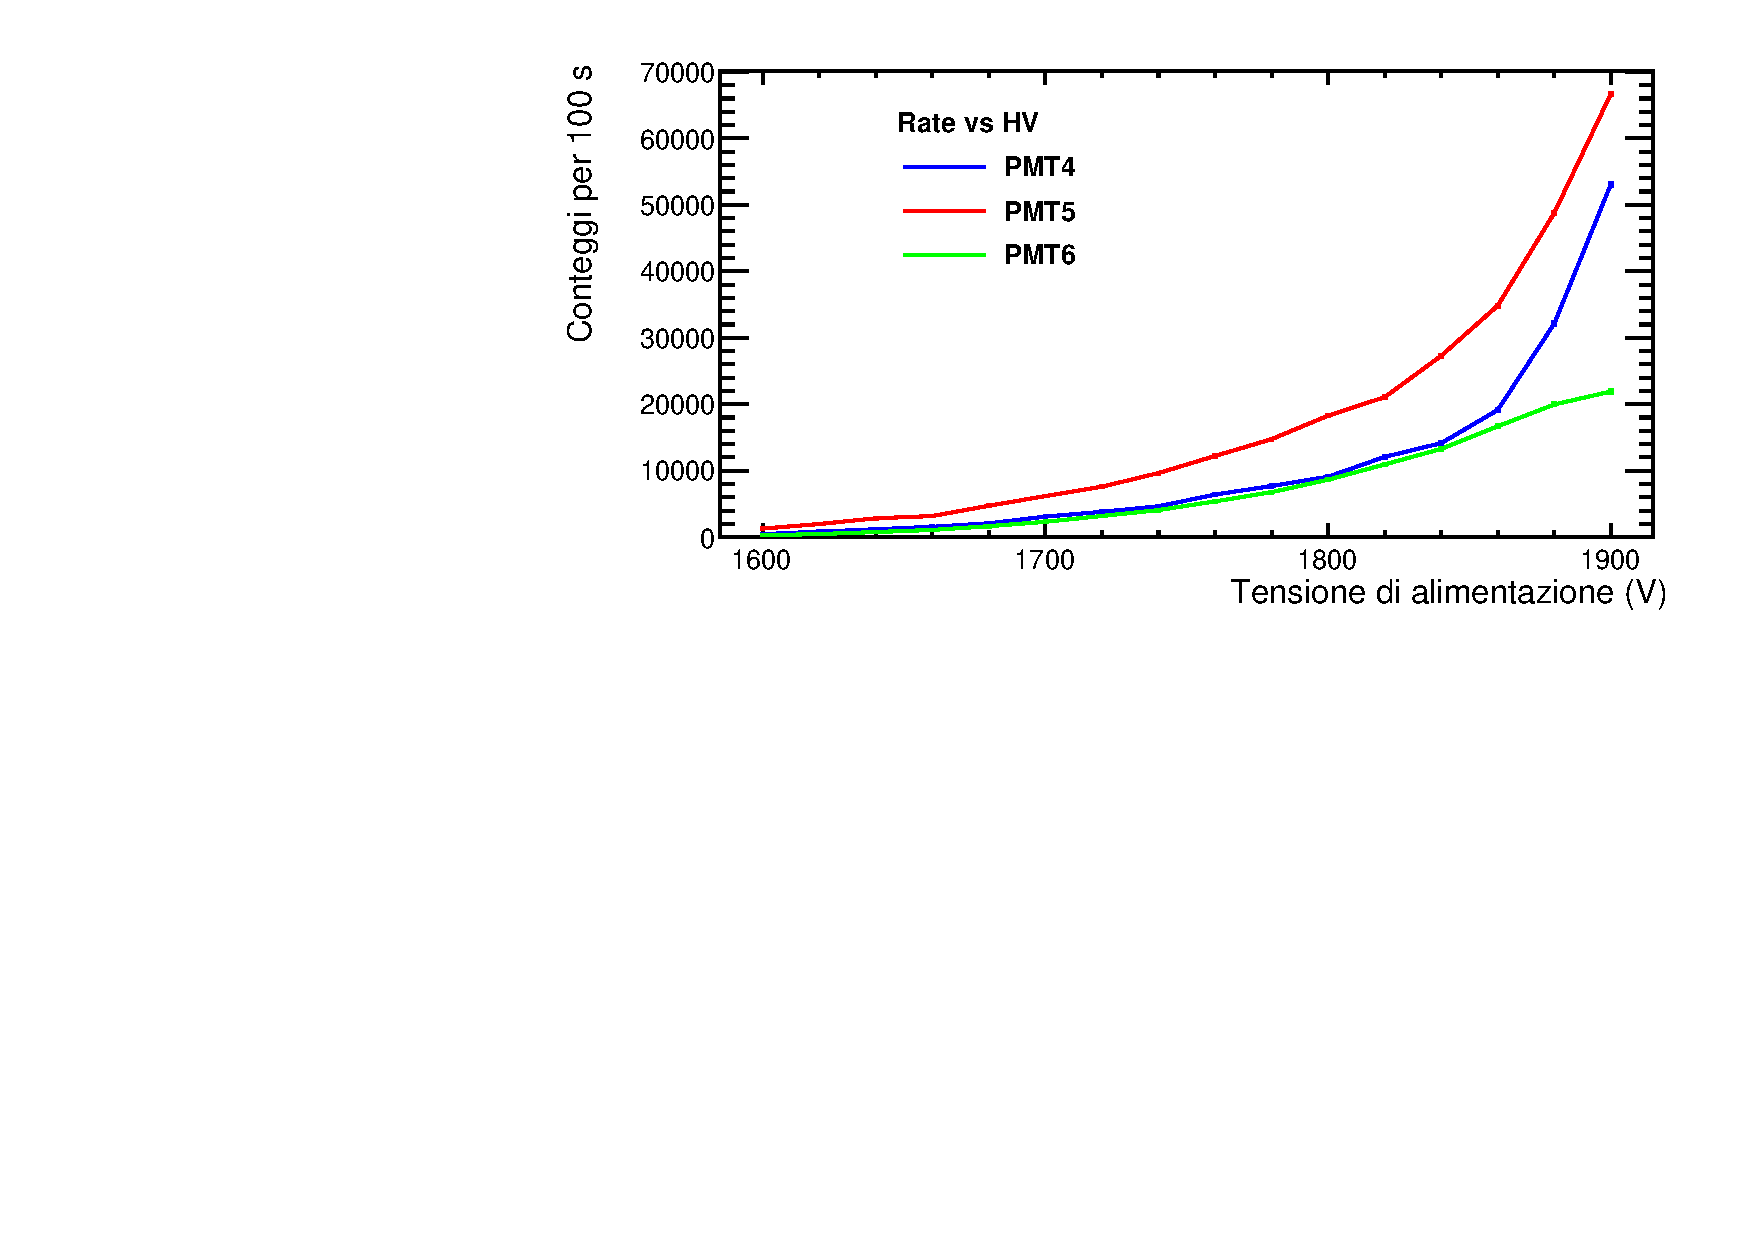
\includegraphics[width=\textwidth]{fig/rate-hv}
\caption{Numeri di conteggi ogni 100 secondi al variare della tensione di alimentazione dei PMT.}
\label{fig:rate-hv}
\end{figure}
Abbiamo alimentato tutti e 3 PMT con una tensione variabile da 1600 a 1900 mV. Abbiamo collegato il segnale dei 3 PMT ad un contatore passando attraverso un discriminatore per il conteggio degli impulsi.\\

Per questa misura abbiamo impostato la minima soglia possibile per il discriminatore, ovvero 32~mV, allo scopo di ottenere una stima conservativa. 
Abbiamo anche impostato una larghezza del segnale di uscita del discriminatore di 40 ns: in questo modo abbiamo eliminato la possibilità di avere conteggi accidentali causati dai piccoli rimbalzi successivi al segnale principale. 

Il grafico in figura~\ref{fig:rate-hv} mostra il numero dei conteggi in funzione della tensione di alimentazione. Si può osservare come i PMT 4 e 6 mostrano un andamento molto simile mentre il PMT 5 presenta un tasso di conteggi più elevato.

Da queste misure risulta difficile individuare un plateau, ma le abbiamo utilizzate in seguito per scegliere punti di lavoro che presentassero una variazione minima del tasso dei conteggi in funzione di variazioni della tensione di alimentazione.

Il numero dei conteggi è molto variabile e non ci permette di stabilire una relazione col numero di raggi cosmici attesi. D'altra parte ci aspettiamo che un singolo scintillatore presenti una quantità di conteggi dovuti al rumore di fondo molto maggiore del numero di conteggi dovuti al passaggio di particelle ionizzanti, ed è per questo che ci aspettiamo tassi di conteggi molto elevati.

\subsection{Calibrazione delle coincidenze}
\begin{table}
\centering
\begin{tabular}{|c|c|c|c|}
\hline
\textbf{HV (V)} & \textbf{PMT4 (Conteggi)} & \textbf{PMT6 (Conteggi)} & \textbf{Coincidenze casuali attese} \\
\hline 
1600 & 451 & 281 & 1.27e-06 \\
\hline
1620 & 832 & 470 & 3.91e-06 \\
\hline
1640 & 1189 & 772 & 9.18e-06 \\
\hline
1660 & 1562 & 1088 & 1.70e-05 \\
\hline
1680 & 2084 & 1654 & 3.45e-05 \\
\hline
1700 & 3095 & 2313 & 7.16e-05 \\
\hline
1720 & 3815 & 3189 & 1.22e-04 \\
\hline
1740 & 4644 & 4074 & 1.89e-04 \\
\hline
1760 & 6408 & 5385 & 3.45e-04 \\
\hline
1780 & 7698 & 6775 & 5.22e-04 \\
\hline
1800 & 9093 & 8648 & 7.86e-04 \\
\hline
1820 & 12081 & 10945 & 1.32e-03 \\
\hline
1840 & 14148 & 13284 & 1.88e-03 \\
\hline
1860 & 19136 & 16686 & 3.19e-03 \\
\hline
1880 & 32146 & 19968 & 6.42e-03 \\
\hline
1900 & 53110 & 21913 & 1.16e-02 \\
\hline

\end{tabular} 
\caption{Calcolo delle coincidenze casuali attese sul numero di conteggi acquisiti per 100 secondi al variare della tensione di alimentazione}
\label{tab:random_coincidence}
\end{table}

\begin{figure}
\centering
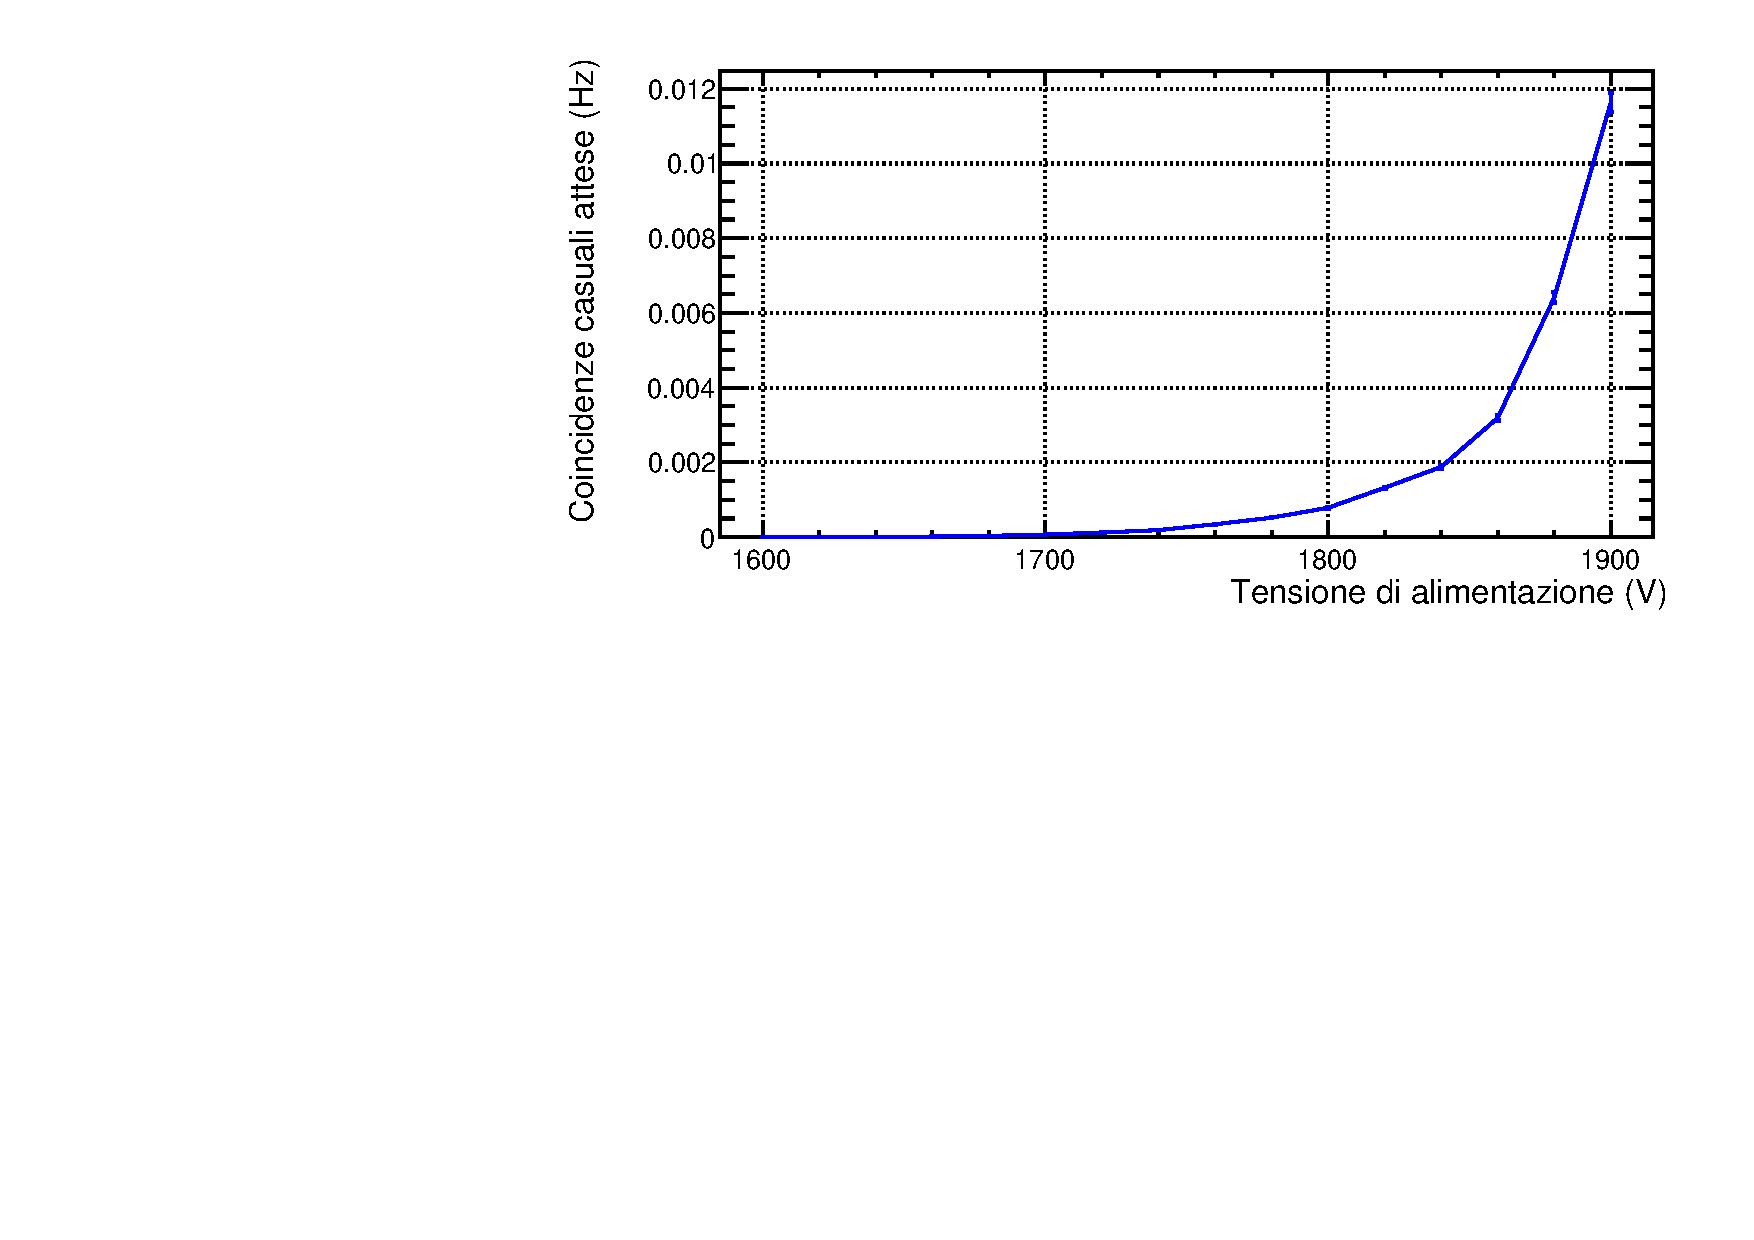
\includegraphics[width=\textwidth]{fig/random_coincidence}
\caption{Calcolo delle coincidenze casuali attese per i PMT4 e 6 in funzione della tensione di alimentazione, fatto sui conteggi acquisiti per 100 secondi. Vedi tabella~\ref{tab:random_coincidence}.}
\label{fig:random_coincidence}
\end{figure}

\begin{figure}
\centering
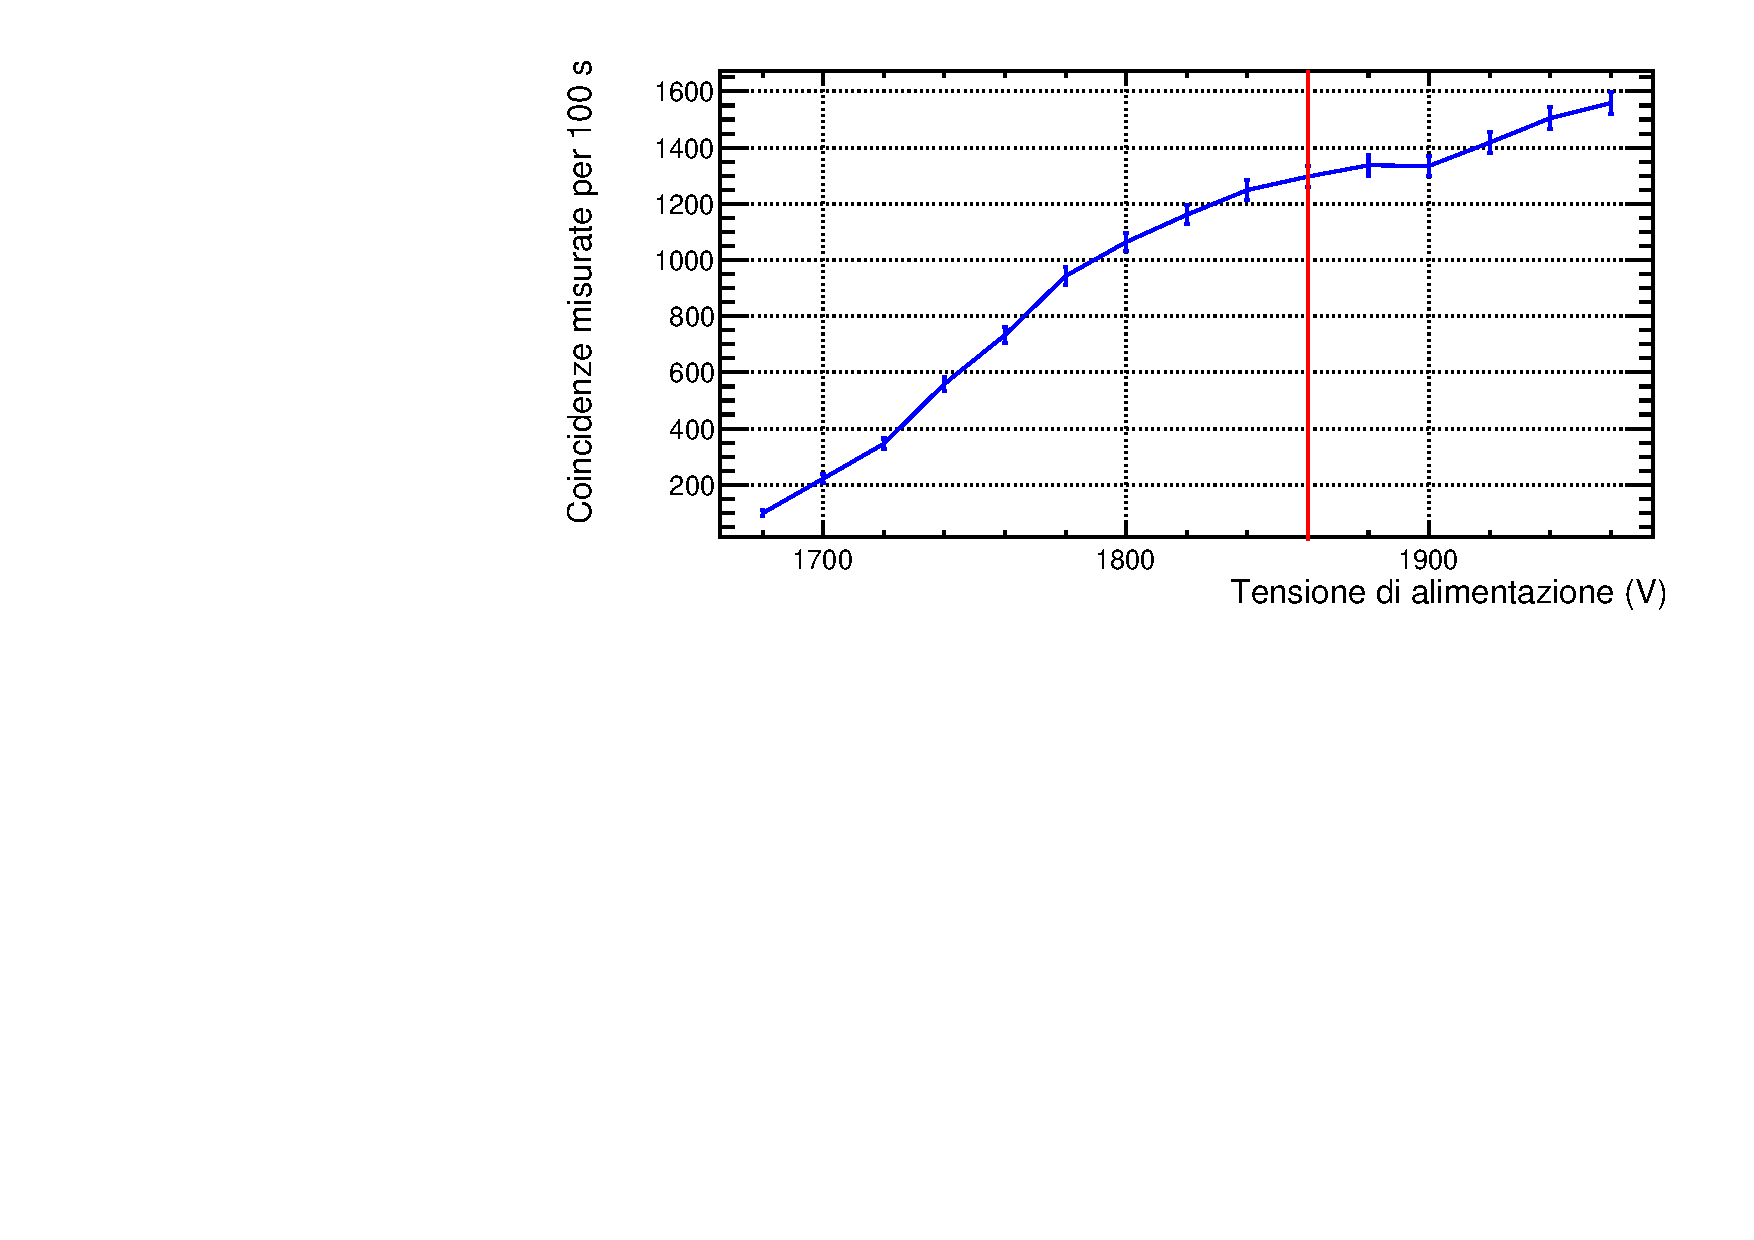
\includegraphics[width=\textwidth]{fig/coincidence}
\caption{Misura delle coincidenze per i PMT4 e 6 in funzione della tensione di alimentazione. Acquisizione di 100 secondi. Data la natura Poissoniana della distribuzione l'errore sui conteggi è stato calcolato come $\sqrt{R}$. Evidenziato in rosso il punto di ascisse 1860 V.}
\label{fig:coincidence}
\end{figure}

Utilizzando i dati in tabella~\ref{tab:random_coincidence}, abbiamo calcolato il tasso di coincidenze casuali attese tra il PMT 4 e 6. In questo modo abbiamo stabilito che mantenendoci al di sotto di una soglia di alimentazione di 1900 V il numero di coincidenze casuali non influisce in maniera significativa sul conteggio di coincidenze reali che ci aspettiamo. 

Il calcolo è stato effettuato considerando una larghezza del segnale del discriminatore di 50 ns, e utilizzando la formula:
\begin{equation}
R_{c} = R_{4}*R_{6}*\Delta t
\label{eq:random_coincidence}
\end{equation}
Con $R_{c}$ uguale al tasso di coincidenze casuali attese, $R_{4,6}$ i conteggi al secondo misurati sul PMT 4 e 6, e $\Delta t = 100$~ns (pari alla somma della larghezza del segnale dei due discriminatori collegati in serie ai PMT) .

Gli errori sui conteggi sono stati calcolati utilizzando la formula:
\begin{equation}
\sigma_{R_{c}} = R_{c} \times{\sqrt{\frac{1}{R_{4}} + \frac{1}{R_{6}} + \left( \frac{\sigma_{t}}{\Delta t} \right)^2}  }
\end{equation}
con $\sigma_{t} = 5$~ns, mentre i conteggi seguono la distribuzione di Poisson e di conseguenza assegnamo $\sqrt{R}$ come incertezza.

A questo punto abbiamo effettuato la misura delle coincidenze in funzione della tensione di alimentazione sui PMT 4 e 6, per trovare un punto di plateau da poter utilizzare per la misura di efficienza del PMT 5.
In questo caso abbiamo deciso di impostare una soglia di 60 mV per limitare il rumore mantenendo comunque il segnale ad un'ampiezza misurabile. 

I risultati di questa misura si possono osservare in figura~\ref{fig:coincidence}. \`E ben visibile un plateau ad una tensione di alimentazione di circa 1860 V.	


\subsubsection{Curva di cavo}
\begin{figure}
\centering
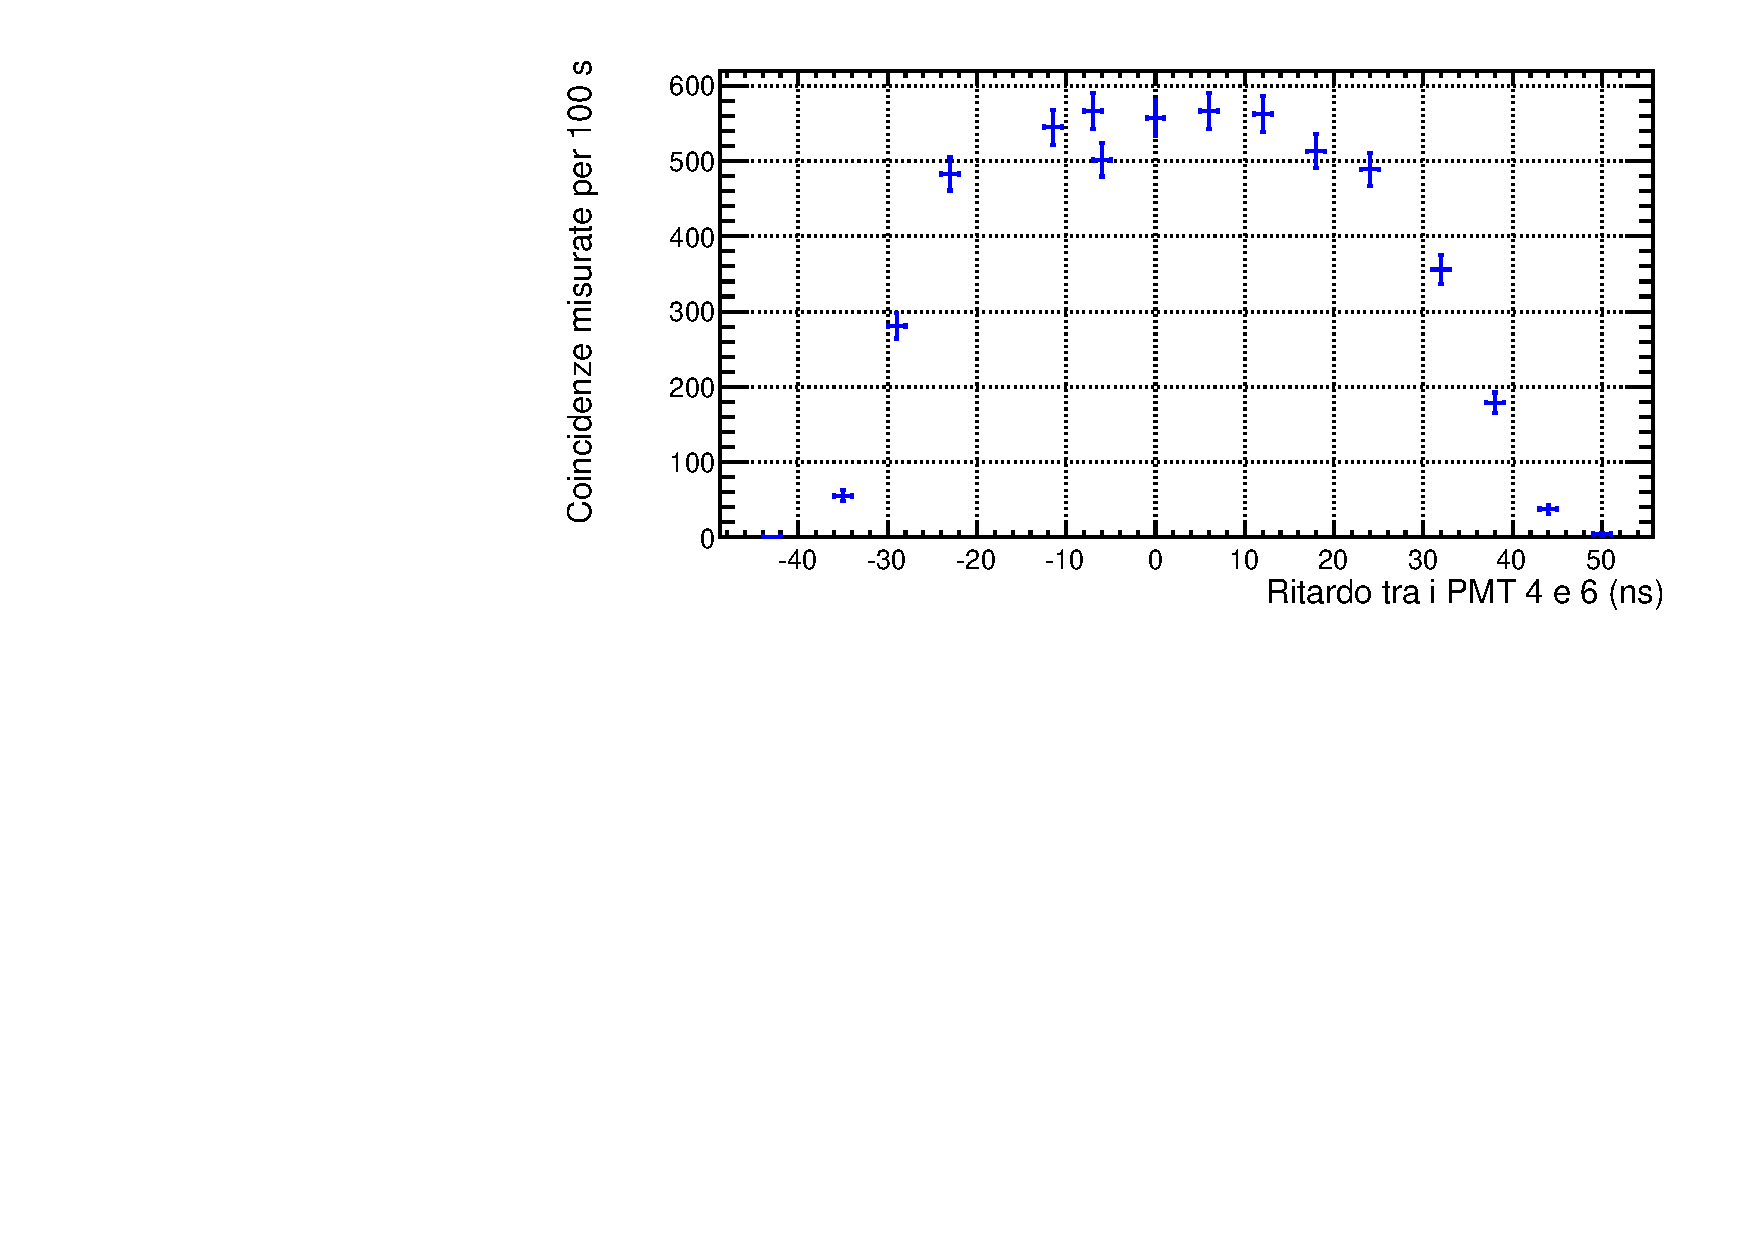
\includegraphics[width=\textwidth]{fig/delay_curve}
\caption{Misura delle coincidenze per i PMT4 e 6 in funzione del ritardo di cavo. Acquisizione di 100 secondi.}
\label{fig:delay_curve}
\end{figure}
Abbiamo realizzato una curva di cavo tra i PMT4 e 6 per assicurarci che i segnali provenienti dai due PMT giungano al modulo delle coincidenze con un ritardo inferiore alla larghezza dei segnali in uscita dei due discriminatori impostata a $t = 50$ ns. 

In figura~\ref{fig:delay_curve} si possono osservare i risultati. La forma quadra del grafico è compatibile con le nostre attese, la larghezza del plateau ci consente di tenerci al riparo da possibili errori dovuti ad oscillazioni nella larghezza del segnale di uscita dei discriminatori. 

Il fatto che la curva sia leggermente spostata verso destra rispetto allo zero potrebbe suggerire l'idea di aggiungere un po' di ritardo tra i due segnali, ma non lo abbiamo comunque ritenuto necessario.
\subsubsection{Misura delle coincidenze casuali}
Abbiamo effettuato una misura delle coincidenze casuali aumentando il ritardo tra i segnali del PMT 4 e 6 ben oltre i valori suggeriti dalla curva in figura~\ref{fig:delay_curve}, in modo da abbattere il numero di coincidenze reali. Considerando che ci aspettavamo un numero di coincidenze casuali molto basse, abbiamo acquisito i dati per un periodo molto più lungo delle precedenti misure.

Il risultato ottenuto visibile in tabella~\ref{tab:random_coincidence_mesured}. Otteniamo un risultato di un ordine di grandezza superiore la nostra stima, quindi è possibile che in questo caso abbiamo sottostimato l'errore. 

\begin{table}
\centering
\begin{tabular}{|c|c|c|c|c|}
\hline 
tempo (s) & Coincidenze & Tasso Coincidenze Casuali (Hz) & Tasso atteso (Hz) \\ 
\hline 
24450 & 1391 & 0.057 & 0.0035\\ 
\hline 
\end{tabular} 
\caption{Misura coincidenze casuali tra PMT 4 e 6, alimentati entrambi con una tensione di 1870 V e con una soglia di 70 mV. Il tasso atteso è stato calcolato secondo la formula~\ref{eq:random_coincidence} .}
\label{tab:random_coincidence_mesured}
\end{table}

\section{Misura dell'efficienza}
\note{definizione dell'efficienza}
\subsection{Risultati}
\label{sec:efficienza} 

%%%%%%%%%%%%%%%%%%%%%%%%%%%%%%%%%%%%%%%%%%%%%%%%%%%%%%%%%%%%%%%%%%%%%%%%%%%%%%%%
%%%%%%%%%%%%%%%%%%%%%%%%%%%%%%%%%%%%%%%%%%%%%%%%%%%%%%%%%%%%%%%%%%%%%%%%%%%%%%%%
%%%%%%%%%%%%%%%%%%%%%%%%%%%%%%%%%%%%%%%%%%%%%%%%%%%%%%%%%%%%%%%%%%%%%%%%%%%%%%%%

\section{Conclusioni}
%%%%%%%%%%%%%%%%%%%%%%%%%%%%%%%%%%%%%%%%%%%%%%%%%%%%%%%%%%%%%%%%%%%%%%%%%%%%%%%%
%%%%%%%%%%%%%%%%%%%%%%%%%%%%%%%%%%%%%%%%%%%%%%%%%%%%%%%%%%%%%%%%%%%%%%%%%%%%%%%%
%%%%%%%%%%%%%%%%%%%%%%%%%%%%%%%%%%%%%%%%%%%%%%%%%%%%%%%%%%%%%%%%%%%%%%%%%%%%%%%%

%\appendix


\end{document}
